\documentclass[10pt]{beamer}
\usetheme{Warsaw}
\usetheme{AnnArbor}
\usecolortheme{beaver}
\usepackage{graphicx}
\usepackage{tikz}
\usetikzlibrary{fadings}

\title{Linux Power!}
\subtitle{(From a view of a PMIC vendor)}
\author{Matti Vaittinen}
\institute{ROHM Semiconductors}
\date{Jan 10 2023}

\begin{document}

%-------------- title
\begin{frame}
	\titlepage

\end{frame}

%-------------- topic page

\begin{frame}{Topics}
	\begin{enumerate}
		\item What and Why is a PMIC?
		\item Regulator provider/consumer
		\item Monitoring for abnormal conditions
		\item Setting safety limits
		\item A helper for sending notifications for “anomalies”
	\end{enumerate}
\end{frame}

%-------------- about me page

\begin{frame}{About Me}
	\begin{columns}
	\column{0.58\linewidth}
		\begin{itemize}
			\item Matti Vaittinen
			\item Kernel/Diver developer at RPHM Semiconductor
			\item Worked at Nokia BTS projects (networking, clock \& sync) 2005 – 2017
			\item Currently mainly developing/maintaining upstream Linux device drivers for ROHM ICs
		\end{itemize}
	\column{0.38\linewidth}
		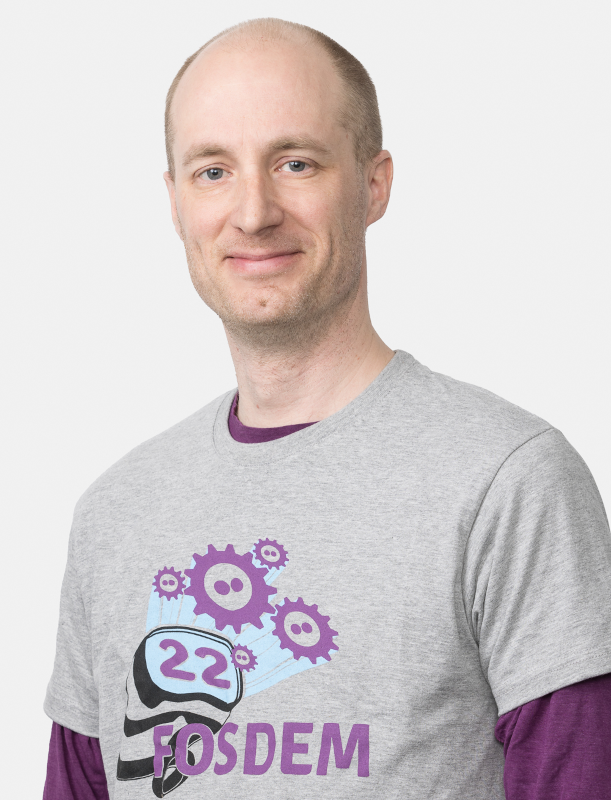
\includegraphics[width=1\linewidth]{me.png}
		%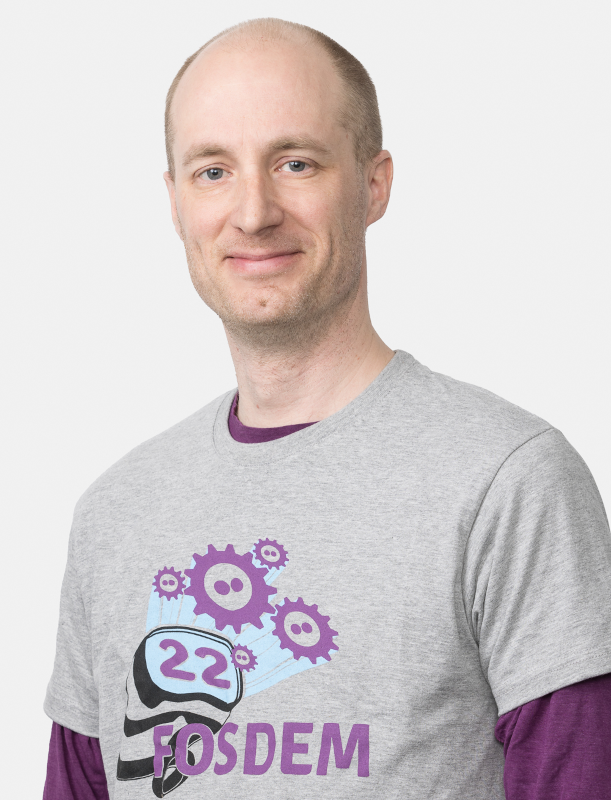
\includegraphics[width=.8\linewidth]{me.png}
	\end{columns}
\end{frame}

%-------------- Powering a processor page

%Arrow style for all of the drawings
\tikzstyle{arrow} = [thick,->,>=stealth]

%Large SOC/PSY boxes
\tikzstyle{psys} = [rectangle, rounded corners, minimum width=3cm, minimum height=3cm,text centered, text width=3cm, draw=black, fill=red!30]
\tikzstyle{socs} = [rectangle, rounded corners, minimum width=3cm, minimum height=3cm,text centered, text width=3cm, draw=black, fill=green!30]

\begin{frame}[t]{Powering a processor}\vspace{4pt}

\begin{itemize}
	\item Processor and peripherals need power
	\item Can be as simple as a dummy DC power source with correct voltage
\end{itemize}


\vfill
\centering
%\begin{minipage}[c]{.5\textwidth}
\begin{minipage}[c]{.75\textwidth}
%  \flushright

\begin{tikzpicture}[node distance=5cm]
	\node (psy) [psys] {DC-source};
	\node (soc) [socs, right of=psy] {SOC};
	\draw [arrow] (psy) -- node[anchor=south] {+5V} (soc);
%  \filldraw[fill=green] (0,0) -- (1,0) -- (1,1) -- (0,1) -- cycle;
  %\fill[green] (90:2) -- (210:2) -- (-30:2) -- cycle;
%  \fill[blue,path fading=west] (80:4) -- (210:4) -- (-30:4) -- cycle;
%\fill[red,path fading=south] (80:4) -- (210:4) -- (-30:4) -- cycle;
\end{tikzpicture}
\end{minipage}
\end{frame}

%-------------- Powering a modern SOC page

%Small PSY clk and SOC boxes
\tikzstyle{s_psys} = [rectangle, rounded corners, minimum width=2cm, minimum height=0.5cm,text centered, text width=2cm, draw=black, fill=red!30]
\tikzstyle{s_clk} = [rectangle, rounded corners, minimum width=2cm, minimum height=0.5cm,text centered, text width=2cm, draw=black, fill=orange!40]
\tikzstyle{s_socs} = [rectangle, rounded corners, minimum width=2.5cm, minimum height=3cm,text centered, text width=2.5cm, draw=black, fill=green!30]

\begin{frame}{Powering a modern SOC 1/2}
	\begin{columns}
	\column{0.3\linewidth}

	 Modern SOCs can require multiple specific voltages

	\column{0.68\linewidth}
%\begin{tikzpicture}[node distance=5cm]
%	\node (nvcc_snvs) [spsys] {LDO1 NVCC SNVS 1.8V};
	%\node (soc) [socs, below of=nvcc_snvs] {SOC};
%	\draw [arrow] (psy) -- node[anchor=south] {+5V} (soc);
%  \filldraw[fill=green] (0,0) -- (1,0) -- (1,1) -- (0,1) -- cycle;
  %\fill[green] (90:2) -- (210:2) -- (-30:2) -- cycle;
%  \fill[blue,path fading=west] (80:4) -- (210:4) -- (-30:4) -- cycle;
%\fill[red,path fading=south] (80:4) -- (210:4) -- (-30:4) -- cycle;
%\end{tikzpicture}

	\begin{tikzpicture}[node distance=0.6cm]
		\node (nvcc_snvs) [s_psys] {LDO1 1.8V};
		\node (vdd_snvs) [s_psys, below of=nvcc_snvs] {LDO2 0.8V};
		\node (rtc_clk) [s_clk, below of=vdd_snvs] {RTC-CLK};
		\node (vdd_soc) [s_psys, below of=rtc_clk] {BUCK1 0.8V};
		\node (vdd_gpu) [s_psys, below of=vdd_soc] {BUCK5 0.9V};
		\node (vdd_phy) [s_psys, below of=vdd_gpu] {LDO4 0.9V};
		\node (vdd_arm) [s_psys, below of=vdd_phy] {BUCK2 0.9V};
		\node (imx8) [s_socs, right of=vdd_arm, xshift=5cm]{SOC};
		\node (vdda_dram) [s_psys, below of=vdd_arm] {LDO3 1.8V};
		\node (nvcc_1v8) [s_psys, below of=vdda_dram] {BUCK7 1.8V};
		\node (nvcc_dram) [s_psys, below of=nvcc_1v8] {BUCK8 1.1V};
		\node (nvcc_3v3) [s_psys, below of=nvcc_dram] {BUCK6 3.3V};
		\node (vdd_phy_1v2) [s_psys, below of=nvcc_3v3] {LDO6 1.2V};
		\node (ldo5) [s_psys, below of=vdd_phy_1v2] {LDO6 1.2V};

		\draw [arrow] (nvcc_snvs) node[anchor=south, xshift=3cm] {\scriptsize NVCC-SNVS} -|  ([xshift=1.6cm] imx8);
		\draw [arrow] (vdd_snvs) node[anchor=south, xshift=3cm] {\scriptsize VDD-SNVS} -| ([xshift=0.5cm] imx8);
		\draw [arrow] (rtc_clk) node[anchor=south, xshift=3cm] {\scriptsize RTC-CLK} -| ([xshift=-0.5cm] imx8);
		\draw [arrow] (vdd_soc) node[anchor=south, xshift=3cm] {\scriptsize VDD-SOC-VDDA-PHY} -| ([xshift=-1cm] imx8);
		\draw [arrow] (vdd_gpu) -- node[anchor=south]{\scriptsize VDD-GPU-VPU-VRAM} (imx8.west|-vdd_gpu) ;
		\draw [arrow] (vdd_phy) -- node[anchor=south] {\scriptsize VDD-PHY} (imx8.west|-vdd_phy);
		\draw [arrow] (vdd_arm) -- node[anchor=south] {\scriptsize VDD-ARM} (imx8.west|-vdd_arm);
		\draw [arrow] (vdda_dram) -- node[anchor=south] {\scriptsize VDDA-DRAM-VDDA} (imx8.west|-vdda_dram);
		\draw [arrow] (nvcc_1v8) -- node[anchor=south] {\scriptsize NVCC} (imx8.west|-nvcc_1v8);
		\draw [arrow] (nvcc_dram) node[anchor=north, xshift=3cm] {\scriptsize NVCC-DRAM} -| ([xshift=-1cm] imx8);
		\draw [arrow] (nvcc_3v3) node[anchor=north, xshift=3cm] {\scriptsize NVCC-3V3} -| ([xshift=-0.5cm] imx8);

		\draw [arrow] (vdd_phy_1v2) node[anchor=north, xshift=3cm] {\scriptsize VDD-PHY-1V2} -| ([xshift=0.5cm] imx8);
		%\draw [arrow] (vdd_phy_1v2) -| node[anchor=north] {\small VDD-PHY-1V2} ([xshift=0.5cm] imx8);
		\draw [arrow] (ldo5) node[anchor=north, xshift=3cm] {\scriptsize VDD-PHY-1V2} -| ([xshift=1.6cm] imx8);
	\end{tikzpicture}
	\end{columns}
\end{frame}

\begin{frame}{Powering a modern SOC 2/2}
	\begin{columns}
	\column{0.3\linewidth}
		And specific timings...
	\column{0.68\linewidth}
		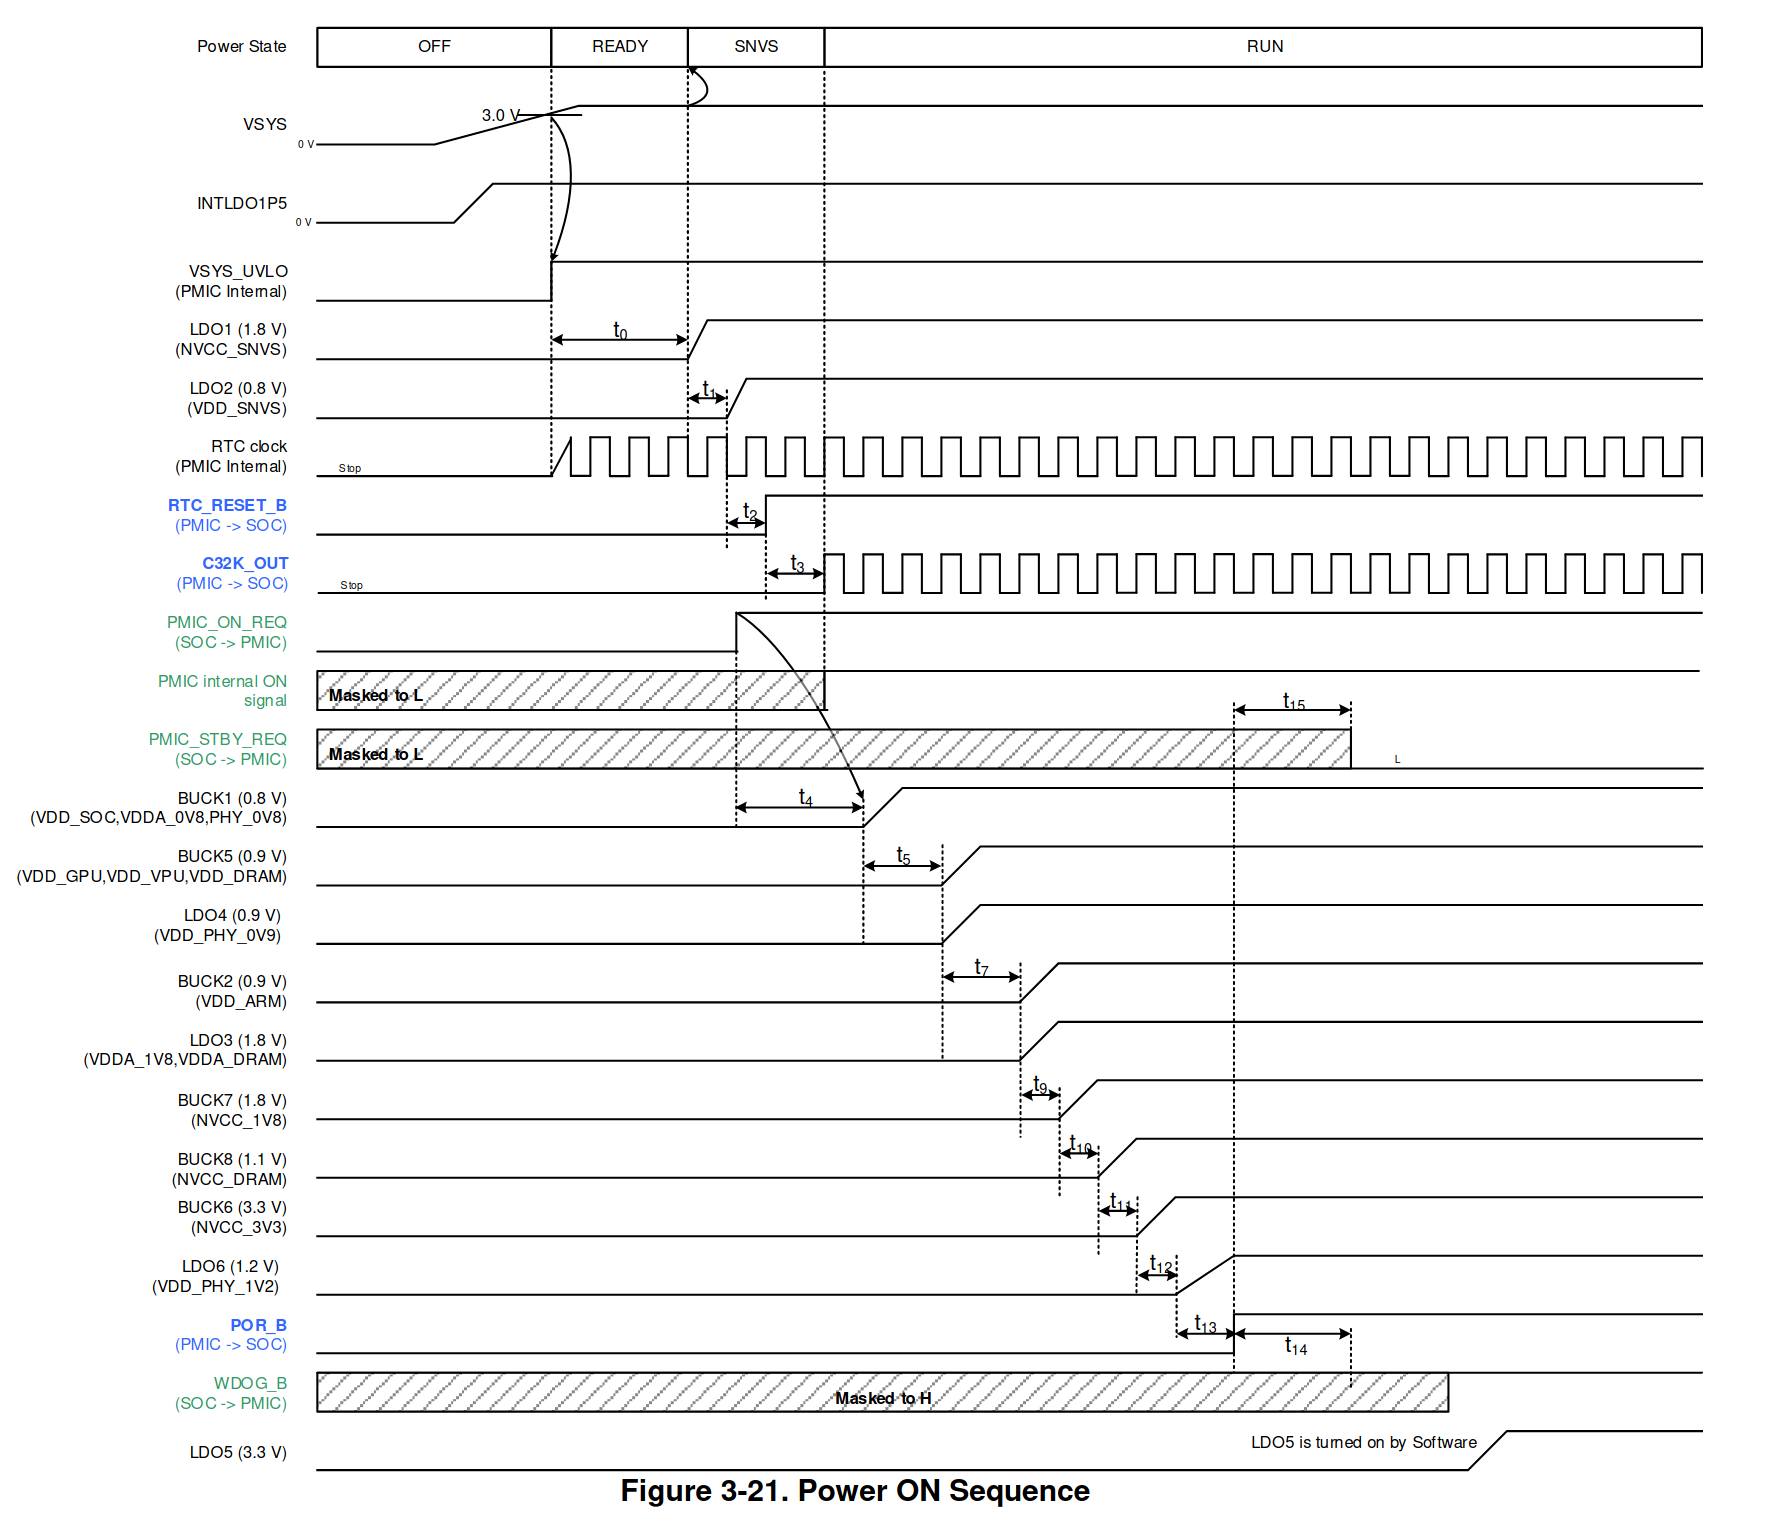
\includegraphics[width=1\linewidth]{BD71847_start_up_seq.png}
	\end{columns}
\end{frame}

\begin{frame}{More control...}
Power savings by:
\begin{itemize}
	\item Shutting down not needed devices
	\item Stand-by state(s)
	\item DVS (Dynamic Voltage Scaling)
\end{itemize}
\end{frame}


\begin{frame}{Automated power on}
Powering-on a system at given time...
\begin{itemize}
	\item RTC
\end{itemize}
...Or by an event
\begin{itemize}
	\item HALL sensor, ...
\end{itemize}
\end{frame}


\begin{frame}{More requirements...}
\begin{itemize}
	\item Battery / charger
	\item Watchdog
	\item Functional-safety
	\begin{itemize}
		\item Voltage monitoring
		\item Current monitoring
		\item Temperature monitoring
	\end{itemize}
\end{itemize}
\end{frame}

\begin{frame}{PMICs}
PMIC - Power Management Integrated Circuit
\begin{itemize}
	\item Multiple DC sources with specific start-up / shut-down sequence
	\item Voltage control
	\item Functional-safety
	\item Auxiliary blocks to support various needs\\ [10pt]
\end{itemize}

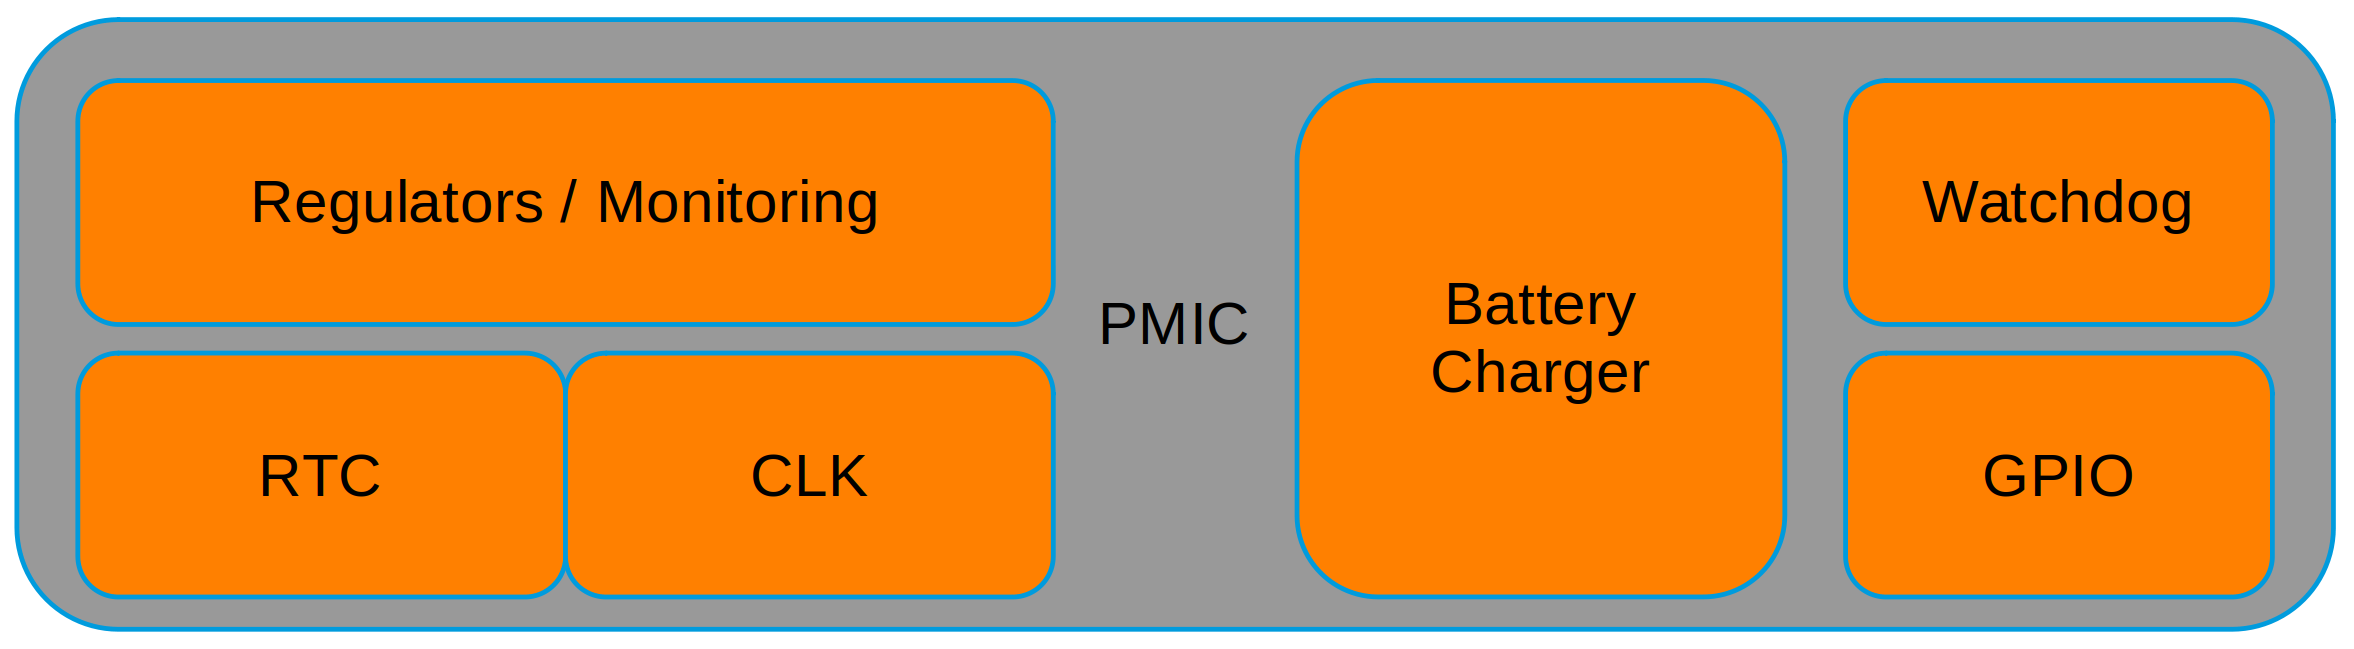
\includegraphics[width=1\linewidth]{pmic_block.png}
\end{frame}


\begin{frame}{Multi Function Devices}
	\begin{columns}
	\column{0.3\linewidth}
Often MFD drivers which allows re-use
	\begin{itemize}
		\item \textbf{Regulator}
		\item RTC
		\item Power supply
		\item Watchdog
		\item GPIO
		\item CLK ...
	\end{itemize}
	\column{0.68\linewidth}
		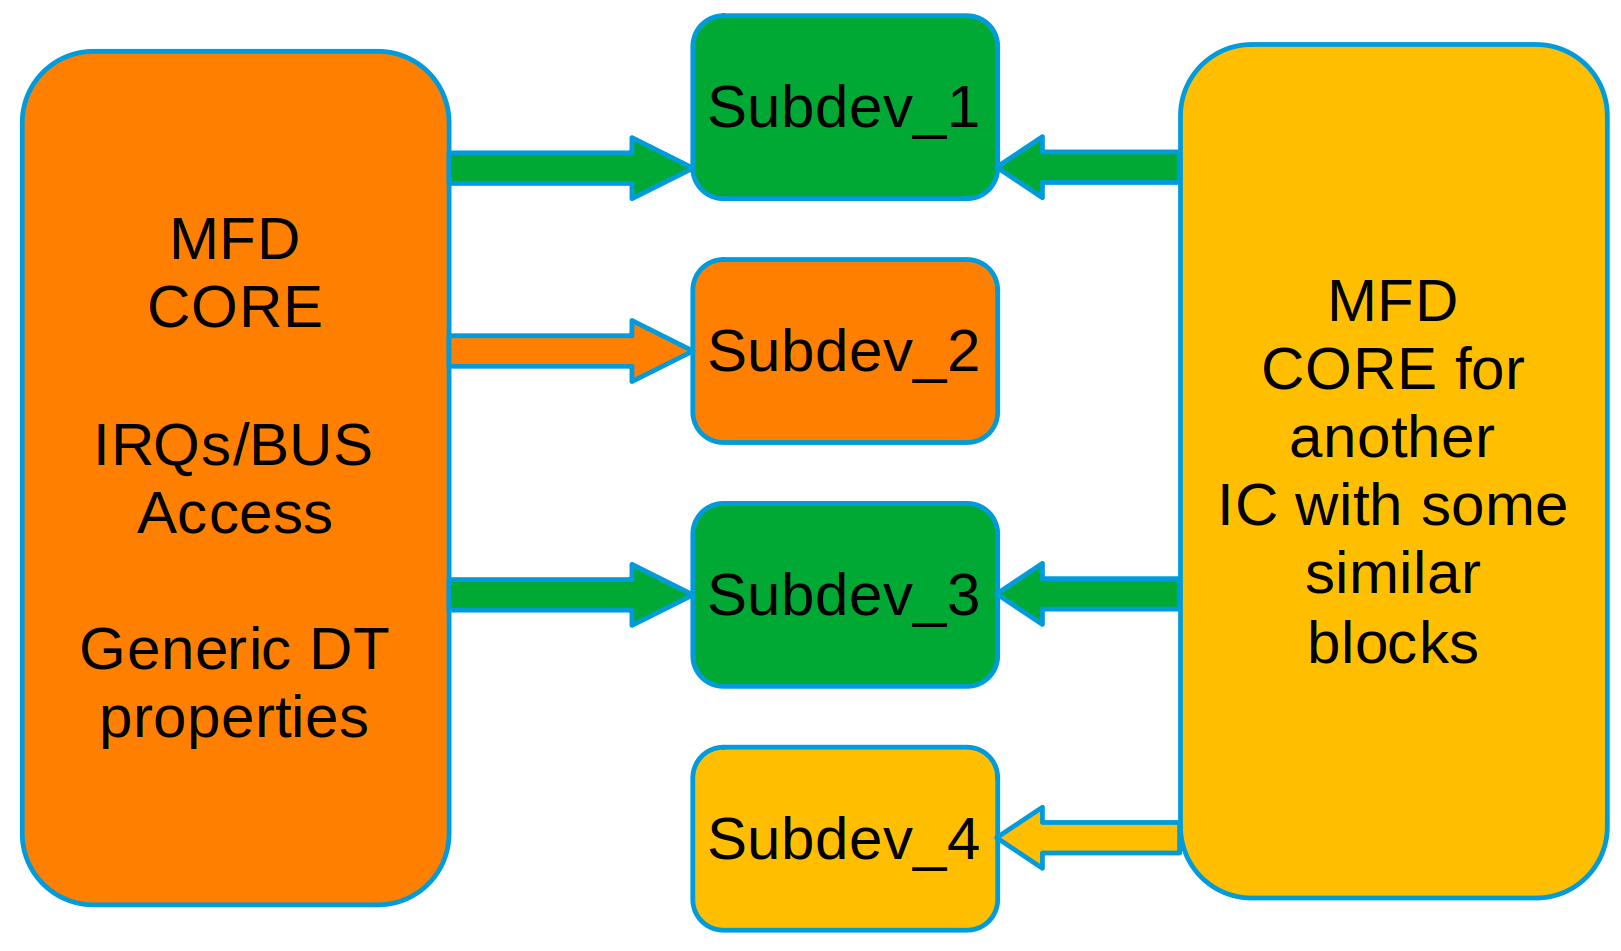
\includegraphics[width=1\linewidth]{MFD_re_use.png}
	\end{columns}
\end{frame}


\begin{frame}{Regulator (provider) and consumer}
\begin{itemize}
	\item Provider is driver interfacing the hardware. Eg, sits “below” the regulator framework. Between regulator framework and HW
	\item Consumer is driver who wishes to control the regulator using the regulator framework. Eg, sits “on top of” the regulator framework
	\item PMIC driver is the provider driver (usually just referred as a regulator driver) \\[10pt]
\end{itemize}
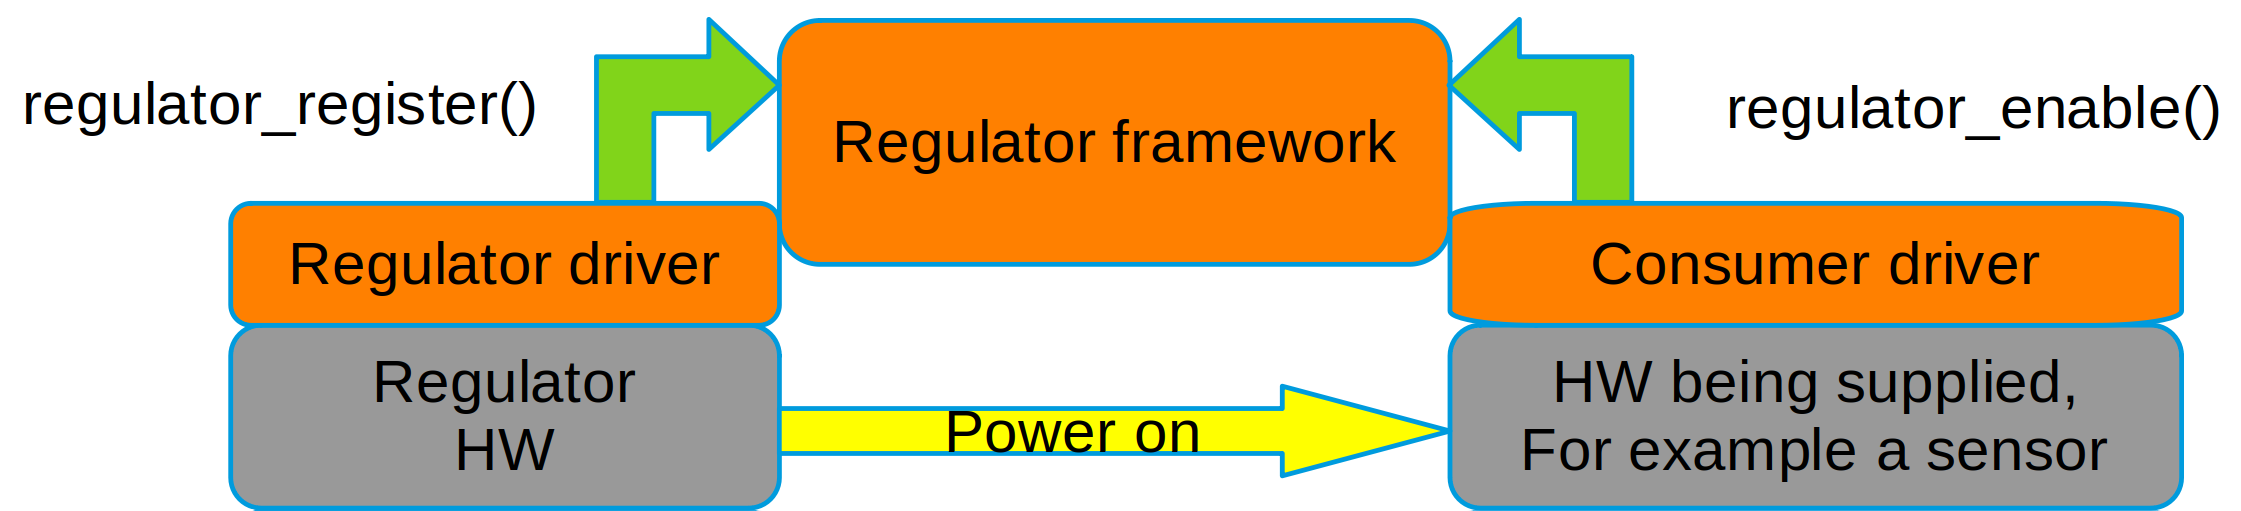
\includegraphics[width=1\linewidth]{regulator_users.png}
\end{frame}

\begin{frame}{Detecting undexpected}
Linux has 3 severity categories
\begin{itemize}
	\item Severity \textcolor{magenta}{\textbf{PROTECTION}}
	\begin{itemize}
		\item Unconditional \textcolor{magenta}{shutdown by HW}
	\end{itemize}
	\item Severity \textcolor{red}{\textbf{ERROR}}
	\begin{itemize}
		\item \textcolor{red}{Irrecoverable error,} system not expected to be usable. Error handling by software.
	\end{itemize}
	\item Severity \textcolor{orange}{\textbf{WARNING} - NEW(ish)}
	\begin{itemize}
		\item \textcolor{orange}{Something is off-limit,} system still usable but a recovery action should be taken to prevent escalation to errors
	\end{itemize}
\end{itemize}
\end{frame}



\end{document}